%% MLMI 2026 variant WITH speaker notes.
%% Each slide is followed by a full page of speaker notes.
%% Compile: pdflatex slides_MLMI_notes.tex  (twice for frame numbers)

\PassOptionsToClass{notes=onlyslideswithnotes}{beamer}

\documentclass[10pt,aspectratio=169]{beamer}

\usetheme{default}
\usecolortheme{seahorse}
\setbeamertemplate{navigation symbols}{}
\setbeamerfont{frametitle}{size=\large,series=\bfseries}
\setbeamerfont{title}{size=\Large,series=\bfseries}

\usepackage{graphicx}
\usepackage{amsmath,amssymb}
\usepackage{booktabs}
\usepackage{xcolor}
\usepackage{tikz}
\usepackage{pgfpages}

\definecolor{accent}{HTML}{C44E52}
\definecolor{good}{HTML}{4C7AB0}

%% Show notes on the right half of a widescreen page.
\setbeameroption{show notes on second screen=right}

%% ---- Conference-specific ----
\newcommand{\confname}{MLMI 2026}
\newcommand{\conflong}{9th Int.\ Conf.\ on Machine Learning and Machine Intelligence}
\newcommand{\confvenue}{Tokyo, Japan}
\newcommand{\confdate}{July 19, 2026}
\newcommand{\confpaperid}{Paper EL0079-A}
%% -----------------------------

\setbeamertemplate{footline}{%
  \leavevmode%
  \hbox{%
    \begin{beamercolorbox}[wd=.6\paperwidth,ht=2.4ex,dp=1ex,leftskip=1em]{author in head/foot}%
      \usebeamerfont{author in head/foot}\confname\ \textbar\ \confvenue\ \textbar\ \confdate%
    \end{beamercolorbox}%
    \begin{beamercolorbox}[wd=.4\paperwidth,ht=2.4ex,dp=1ex,rightskip=1em]{author in head/foot}%
      \usebeamerfont{author in head/foot}\hfill\confpaperid\ \textbar\ \insertframenumber%
    \end{beamercolorbox}%
  }%
  \vskip0pt%
}

\title{Beyond Representation:\\ Index Structure Limitations in Dense Retrieval}
\author{Alessandro Magnani}
\institute{\conflong\\ \confname\ \textbar\ \confvenue}
\date{\confdate}

\begin{document}
%% Shared slide body. Include from slides_MLMI.tex or slides_AMLDS.tex.
%% Expects the following macros to be defined by the wrapper before \input:
%%   \confname   e.g. "MLMI 2026"
%%   \confvenue  e.g. "Tokyo, Japan"
%%   \confdate   e.g. "July 19, 2026"

%% =====================================================================
\begin{frame}[plain]
  \titlepage
\end{frame}

%% =====================================================================
\begin{frame}{Why this talk: can we drop the sparse side?}
  \textbf{Production retrieval today is \alert{hybrid}}: a dense embedding index
  (HNSW / IVF) \emph{plus} an inverted index (BM25). Two stores, two scoring
  paths, extra ops.

  \medskip
  \textbf{The tempting question}: could a pure-dense stack replace hybrid?
  Simpler, one index, one score.

  \medskip
  Two things have to hold:
  \begin{itemize}
    \item \textbf{Bottleneck 1 --- representation.}
          Can the embedding \emph{encode} what BM25 encodes?
          Well-studied: Tay et al.\ 2020, Fan et al.\ 2022 --- capacity grows with $d$.
    \item \textbf{Bottleneck 2 --- indexing.}
          Even if the embedding is capable, can an \emph{ANN index} still find it?
          \alert{This talk. Largely unstudied.}
  \end{itemize}

  \vspace{0.5em}
  \begin{block}{Headline}
    Switching Flat $\to$ HNSW forfeits \textbf{$\sim 63\%$} of achievable Recall@10
    on identifier queries---and less than $2\%$ on standard queries.
    Same embedding. The index alone.
  \end{block}
\end{frame}

%% =====================================================================
\begin{frame}{The population that pays the bill: ``spear-fishing'' queries}
  \begin{block}{Working definition}
    Queries whose relevance hinges on a single, low-frequency, high-IDF token:
    identifiers (SKUs, part numbers), rare terms, precise named entities.
  \end{block}

  \begin{itemize}
    \item Small fraction of traffic, but operationally critical:
          failed spear-fishing $\Rightarrow$ empty result pages, abandoned carts,
          broken RAG lookups.
    \item BM25 handles them trivially (exact token match).
    \item If pure dense is going to replace hybrid, it has to hold up \emph{here}.
    \item Our three query subsets: \textbf{standard} (control),
          \textbf{rare} ($\le 5$ docs), \textbf{ID} (extreme case: doc identifier
          as query).
  \end{itemize}
\end{frame}

%% =====================================================================
\begin{frame}{Quick primer: what is an IVF index?}
  \textbf{IVF} (Inverted File) --- the standard partition-based ANN index.
  \begin{enumerate}
    \item Cluster the corpus into $N$ cells (k-means). Each cell has a
          \emph{centroid} $c$.
    \item At query time: score the query against all $N$ centroids;
          keep the top $n_{\text{probe}}$.
    \item Only search documents inside those $n_{\text{probe}}$ cells.
  \end{enumerate}

  \begin{center}
    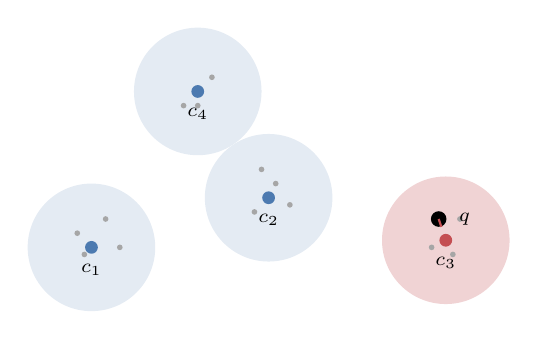
\begin{tikzpicture}[scale=0.9]
      \fill[good!15] (0.5,0.5) circle (0.9);
      \fill[good!15] (3.0,1.2) circle (0.9);
      \fill[accent!25] (5.5,0.6) circle (0.9);
      \fill[good!15] (2.0,2.7) circle (0.9);
      \foreach \x/\y in {0.4/0.4, 0.7/0.9, 0.3/0.7, 0.9/0.5,
                         2.8/1.0, 3.1/1.4, 3.3/1.1, 2.9/1.6,
                         5.3/0.5, 5.7/0.9, 5.6/0.4,
                         1.8/2.5, 2.2/2.9, 2.0/2.5}
        \fill[gray!70] (\x,\y) circle (0.04);
      \fill[good] (0.5,0.5) circle (0.09);
      \fill[good] (3.0,1.2) circle (0.09);
      \fill[accent] (5.5,0.6) circle (0.09);
      \fill[good] (2.0,2.7) circle (0.09);
      \fill[black] (5.4,0.9) circle (0.11);
      \node[right] at (5.55,0.9) {\scriptsize $q$};
      \draw[dashed,accent,thick] (5.4,0.9) -- (5.5,0.6);
      \node[below] at (0.5,0.4) {\scriptsize $c_1$};
      \node[below] at (3.0,1.1) {\scriptsize $c_2$};
      \node[below] at (5.5,0.5) {\scriptsize $c_3$};
      \node[below] at (2.0,2.6) {\scriptsize $c_4$};
    \end{tikzpicture}
  \end{center}

  \vspace{-0.4em}
  \small
  \textbf{Speedup}: $N / n_{\text{probe}}$ fewer distance computations.\quad
  \textbf{Failure mode}: if the relevant cell's centroid is not in the top
  $n_{\text{probe}}$ by query similarity, its documents are \emph{invisible}.
\end{frame}

%% =====================================================================
\begin{frame}{The mechanism: centroid dilution (intuition)}
  A centroid is the \emph{average} of the vectors in its cell.

  \medskip
  \begin{itemize}
    \item A \emph{common} token appears in many docs $\Rightarrow$ contributes
          strongly to the average $\Rightarrow$ shows up in the centroid.
    \item A \emph{rare} token appears in a handful of docs $\Rightarrow$ its
          contribution is averaged \emph{away} $\Rightarrow$ nearly invisible
          in the centroid.
  \end{itemize}

  \medskip
  Now consider a query dominated by that rare token:
  \begin{itemize}
    \item Query vector has huge weight on the rare token direction.
    \item Every centroid --- \emph{including the one containing the relevant docs} ---
          has almost zero weight on that direction.
    \item Result: \alert{all centroids look equally (un)related to the query}.
          Cluster selection becomes essentially random.
  \end{itemize}

  \medskip
  \emph{The failure is not the embedding. It is the averaging step in the index.}
\end{frame}

%% =====================================================================
\begin{frame}{The mechanism: the bound}
  Centroid of cluster $C$:\;
  $c \;=\; \dfrac{1}{|C|}\sum_{d\in C} f(d)$

  \medskip
  For a query $q$ dominated by rare token $t^*$ with IDF-like weight
  $\alpha_{t^*}$ and in-cluster prevalence $p = n_{t^*, C}/(M/N)$:
  \begin{equation*}
    \langle c,\, q\rangle
      \;\approx\; \alpha_{t^*}^2 \, p
      \;=\; \underbrace{\log^2\!\Big(\tfrac{M}{n_{t^*}}\Big)}_{\text{IDF, big for rare}}
            \cdot\underbrace{\frac{n_{t^*, C}}{M/N}}_{\text{prevalence, small for rare}}
  \end{equation*}

  \medskip
  \textbf{JL noise floor}. Any embedding of dimension $d$ obtained by
  Johnson--Lindenstrauss random projection preserves inner products
  \emph{up to} a noise term:
  \begin{equation*}
     \epsilon \;\approx\; \sqrt{\log V / d}
  \end{equation*}
  ($V$ = vocabulary size). Signals weaker than $\epsilon$ are indistinguishable
  from random.

  \medskip
  \alert{The centroid signal is lost whenever $\alpha_{t^*}^2 \, p \;\lesssim\; \epsilon$.}
  \emph{Larger $d$ shrinks $\epsilon$; nothing shrinks the fact that $p$ is small.}
\end{frame}

%% =====================================================================
\begin{frame}{HNSW isn't a way out}
  \textbf{HNSW} is not partition-based --- it is a \emph{layered proximity graph}.
  Greedy descent from a hub node down to the query's local neighborhood.

  \medskip
  \textbf{So why does it fail on the same queries?}
  \begin{itemize}
    \item Graph edges are built from Euclidean distances during insertion.
    \item Dense regions of the embedding space get thick, well-connected
          subgraphs. Rare vectors land in sparse regions --- \emph{few incoming
          edges from any hub}.
    \item Greedy search from a hub cannot reach an orphan node without a long
          detour: it stops at a locally-good but globally-wrong region.
    \item Widening the beam (\texttt{efSearch}) helps --- but with diminishing
          returns.
  \end{itemize}

  \medskip
  \textbf{The pattern is the same}: rare-token vectors are structurally hard
  to \emph{reach}, whether the structure is a partition (IVF) or a graph (HNSW).
  Different mechanism; \alert{same victims}.
\end{frame}

%% =====================================================================
\begin{frame}{Experimental setup (compact)}
  \begin{columns}[T]
    \column{0.55\textwidth}
    \textbf{Datasets} (1{,}000 queries per subset)
    \begin{itemize}
      \item Home Depot (HD): 54{,}667 product titles
      \item MS MARCO Passage v1.1: 82{,}360 passages
    \end{itemize}

    \textbf{Query subsets}
    \begin{itemize}
      \item standard $\;\vert\;$ rare ($\le 5$ docs) $\;\vert\;$ ID
    \end{itemize}

    \column{0.45\textwidth}
    \textbf{Representation}: char-trigram + JL projection,
    $d\in\{256,512,1024\}$, unsupervised.

    \textbf{Indices (FAISS)}: Flat, IVF, HNSW ($M{=}16$, $\text{efC}{=}200$),
    BM25 baseline (Pyserini).
  \end{columns}

  \vspace{0.8em}
  \begin{block}{Why unsupervised trigrams?}
    A supervised encoder abstracts away the lexical detail that \emph{defines}
    spear-fishing queries. To isolate the \emph{index} bottleneck from the
    representation bottleneck we need a representation that provably preserves
    lexical distances (Johnson--Lindenstrauss).
  \end{block}
\end{frame}

%% =====================================================================
\begin{frame}{Headline result: the Flat $\to$ HNSW gap}
  \begin{center}
    \small
    \setlength{\tabcolsep}{6pt}
    \begin{tabular}{llrrrr}
      \toprule
      \textbf{Dataset} & \textbf{Subset} & \textbf{Flat} & \textbf{IVF} & \textbf{HNSW} & \textbf{BM25} \\
      \midrule
      HD       & standard & 0.327 & 0.314 & 0.321 & 0.447 \\
      HD       & rare     & 0.751 & 0.642 & 0.619 & 0.878 \\
      HD       & {\color{accent}\textbf{id}} & {\color{accent}\textbf{0.874}} & 0.590 & {\color{accent}\textbf{0.327}} & 1.000 \\
      \midrule
      MS MARCO & standard & 0.471 & 0.448 & 0.446 & 0.770 \\
      MS MARCO & rare     & 0.205 & 0.187 & 0.166 & 0.688 \\
      MS MARCO & {\color{accent}\textbf{id}} & {\color{accent}\textbf{0.174}} & 0.152 & {\color{accent}\textbf{0.071}} & --- \\
      \bottomrule
    \end{tabular}\\[4pt]
    {\footnotesize Recall@10 at $d{=}1024$, best ANN sweep config.}
  \end{center}

  \vspace{0.4em}
  \begin{itemize}
    \item Relative Flat$\to$HNSW loss:
          HD $\{$standard \textbf{1.8\%}, rare \textbf{17.5\%},
          \alert{id \textbf{62.6\%}}$\}$; MM analogous.
    \item The gap tracks the query population exactly as the theory predicts.
  \end{itemize}
\end{frame}

%% =====================================================================
\begin{frame}{Direct evidence: measure the centroid signal}
  \textbf{For each query}: compute $\langle q,\, c_{\text{rel}}\rangle$
  on the centroid of the query's \emph{relevant} cluster
  (IVF, $n_{\text{list}}{=}500$, $d{=}1024$, HD).

  \begin{columns}[T]
    \column{0.55\textwidth}
    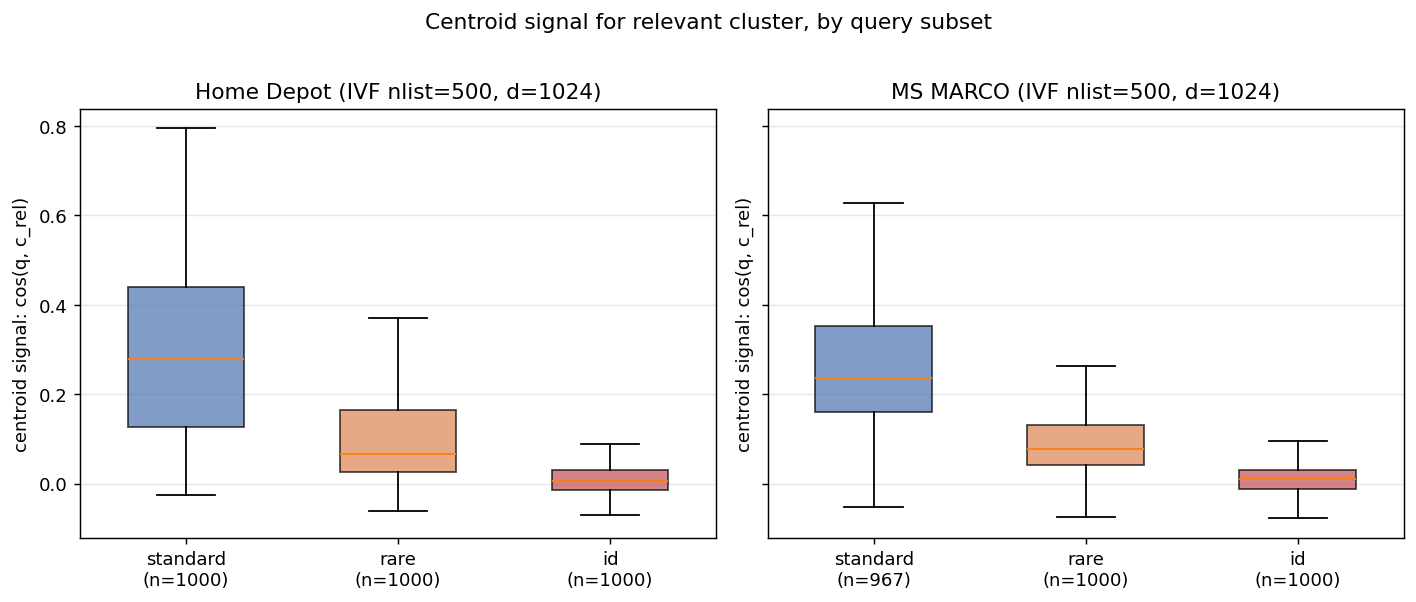
\includegraphics[width=\textwidth]{figures/centroid_signal_by_subset.png}

    \column{0.45\textwidth}
    \small
    \setlength{\tabcolsep}{3pt}
    \begin{tabular}{lrrr}
      \toprule
      Subset & signal & rank & hit@250 \\
      \midrule
      standard & 0.279 & 2   & 97\% \\
      rare     & 0.066 & 69  & 81\% \\
      \alert{id} & \alert{0.007} & \alert{216} & \alert{59\%} \\
      \bottomrule
    \end{tabular}

    \medskip
    \alert{$\sim 40\times$ collapse} of the centroid signal from standard to ID
    --- the correct cluster is buried at rank $\sim 200$.
  \end{columns}

  \medskip
  \small The bound $\langle c,q\rangle \approx \alpha_{t^*}^2 p$ is not just
  suggestive --- it is what we \emph{measure}.
\end{frame}

%% =====================================================================
\begin{frame}{The production-visible symptom}
  \begin{columns}[T]
    \column{0.55\textwidth}
    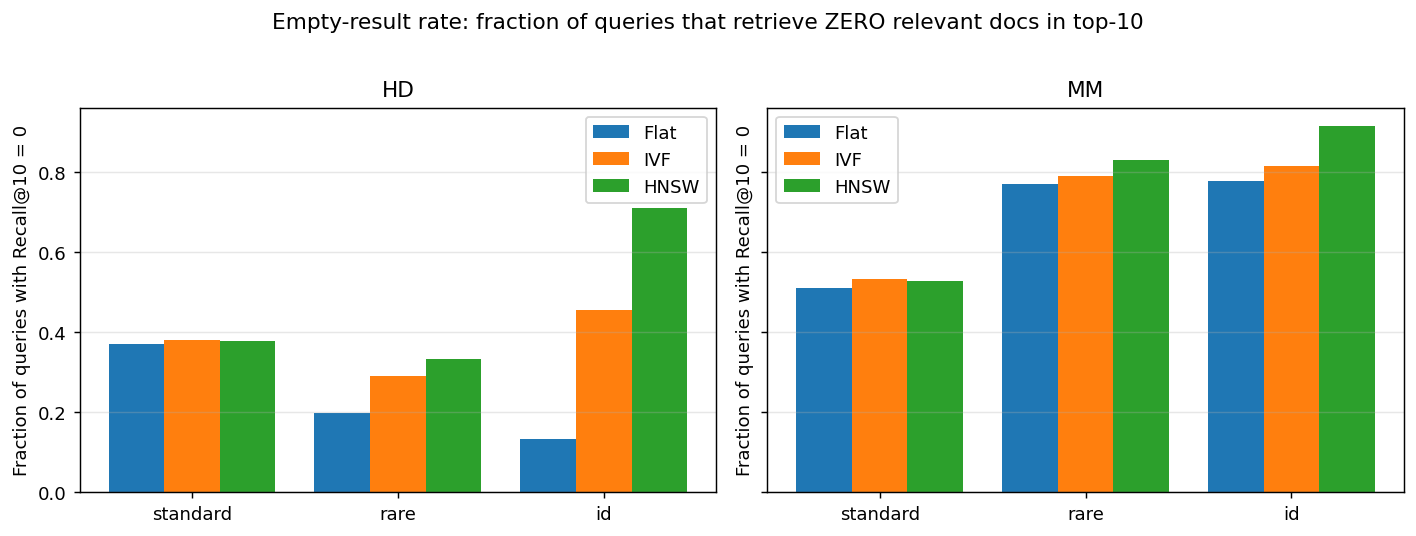
\includegraphics[width=\textwidth]{figures/D_zero_rate.png}

    \column{0.45\textwidth}
    \textbf{Fraction of queries with zero relevant docs in top-10:}
    \begin{itemize}
      \item HD-id: Flat \textbf{13\%} $\to$ HNSW \alert{\textbf{71\%}}
      \item MM-id: Flat \textbf{78\%} $\to$ HNSW \alert{\textbf{92\%}}
      \item Standard: within $\pm 2$ pp on both datasets.
    \end{itemize}

    \medskip
    \textbf{Cost to match Flat recall} (efSearch, HD):
    \begin{itemize}
      \item standard: \textbf{2.7$\times$ faster} than Flat
      \item id: \alert{\textbf{40$\times$ slower}} than Flat
    \end{itemize}
    ANN's speedup evaporates on the population that needs it most.
  \end{columns}
\end{frame}

%% =====================================================================
\begin{frame}{``But learned encoders would fix this''}
  Anticipated question: \emph{do supervised dense encoders escape the issue?}

  \medskip
  Re-ran with \texttt{all-MiniLM-L6-v2} (Sentence-BERT, 384-dim):

  \begin{center}
    \small
    \setlength{\tabcolsep}{6pt}
    \begin{tabular}{llrr}
      \toprule
      Dataset & Subset & Trigram Flat R@10 & \textbf{MiniLM Flat R@10} \\
      \midrule
      HD       & standard & 0.327 & 0.298 \\
      HD       & rare     & 0.751 & 0.428 \\
      HD       & {\color{accent}id} & {\color{good}0.874} & {\color{accent}\textbf{0.010}} \\
      MS MARCO & standard & 0.471 & {\color{good}\textbf{0.894}} \\
      MS MARCO & {\color{accent}id} & {\color{good}0.174} & {\color{accent}\textbf{0.001}} \\
      \bottomrule
    \end{tabular}
  \end{center}

  \vspace{0.5em}
  \begin{itemize}
    \item MiniLM \emph{cannot distinguish identifiers} --- ``12345'' $\approx$ ``67890''.
    \item Representation collapses \emph{before} the index has a chance to bias.
    \item Which is precisely why hybrid retrieval exists.
  \end{itemize}
\end{frame}

%% =====================================================================
\begin{frame}{Takeaways}
  \begin{enumerate}
    \item Production dense retrieval is hybrid for a reason. If you want to
          drop the sparse side, you have to clear \emph{two} bottlenecks, not one.
    \item Bottleneck 1 (representation) is well-studied. Bottleneck 2
          (indexing) is what this paper isolates and quantifies.
    \item Centroid dilution + JL noise floor give a closed-form bound; the
          $\sim 40\times$ centroid-signal collapse from standard to ID is
          exactly what the bound predicts.
    \item HNSW is not a workaround --- the mechanism differs, the victims
          don't.
    \item Practical implication: query-type-aware routing, index-aware
          training, or --- most simply --- keep the sparse side.
  \end{enumerate}

  \vfill
  \begin{center}
    \large
    \textbf{Code \& experiments:} \texttt{github.com/alemagnani/sparse-dense-paper}
  \end{center}
\end{frame}

%% =====================================================================
\begin{frame}[plain]
  \begin{center}
    \vspace{2em}
    {\Huge \bfseries Thank you}\\[1em]
    {\large Questions?}\\[2em]

    \small Alessandro Magnani \;\textbar\; \texttt{ale.magnani@gmail.com}\\
    \confname \;\textbar\; \confvenue \;\textbar\; \confdate
  \end{center}
\end{frame}

\end{document}
